
\section{Detection or identification: RNN as hybrid}

Without changes to the model or the training process, the RNN can be used for both the identification task and the detection task. This is illustrated in the following subsections. First, the RNN is compared against an MLP and CNN in the task of classifying light curve segments as signal or non-signal. Then, we show how the RNN trained for this task can also be used for locating signals in time for arbitrarily sized input light curves. Different network architectures are tested, which serves as a motivation for our choices of the network architecture used in subsequent experiments.

\subsection{Fixed input size, single output}
\label{sec:identification}

As described in Section \ref{eq:objective}, the RNN is trained to classify each data point of a given light curve as signal or non-signal. Recall that we refer to these outputs as the probability time series (PTS). However, in the task of classifying an entire input light curve segment as signal or non-signal, we only need a single output. Two options to obtain a single RNN output for a given input light curve segment are: (i) use the maximum of the PTS for the binary classification of the whole segment; or (ii) train an RNN specifically for this task, while only using the output at the last time step for the binary classification of the segment. We refer to (ii) as the \textit{naive} approach, since this approach does not utilize the full learning potential of the RNN as it only provides a sparse learning signal. 

Two data sets were generated using LCSim, both consisting of 15000 light curve segments for training, 5000 for validation and 5000 for testing. For each split, 50\% of the segments contained at least one transit signal and the other 50\% contained no signals. One data set contained light curve segments consisting of $N=500$ data points, and for the other data set $N = 1500$. In other words, the time spans of segments in each data set were 16.7 and 50 hours respectively. Several models were trained using the training sets, their architectures were determined by inspecting their performances on the validation sets, and only here analyse the performances on the test sets. For each model, an informal search over hyperparameters was performed to determine the final architecture, the process of which is further described in the following.

The MLP is a simple network consisting of several fully-connected (FC) layers. We experimented with different numbers of layers and nodes per layer, and decided on a network consisting of three hidden layers with 128, 64 and 64 nodes respectively. Several variations to these values were tested, but resulted in similar performance. However, the weight decay parameter seemed to be of importance to the performance of the network, as for low values of this parameter the MLP was found to quickly overfit the training data. We therefore used a weight decay of \num{5e-3}. The ReLU activation function is applied between layers and the sigmoid is applied to the final output. Each of the described networks in the following use the same activation functions.

The CNN requires the specification of more hyperparameters. In an attempt of keeping the architecture simple, we found several hyperparameter settings to result in similar performance. In the following we use a CNN with three convolutional layers, consisting of 4, 12 and 1 channels respectively, using kernel sizes of 7, 7 and 3 and a stride of 1 at each layer. After each layer, we apply batch normalization and a max-pooling operation over 3 nodes. The final layer of the network is an FC-layer of 48 nodes. 

For the RNN, GRU was found to produce better and more stable results than LSTM. In Figure \ref{fig:hybrid-gru_architectures} we compare several architectures of the bidirectional GRU with a single layer (bi-GRU-1). The hyperparameters that were varied over were the number of hidden nodes in the recurrent cell, the number of FC-layers that follow the recurrent layer, and the number of nodes per FC-layer. For each set of parameters, the network's performance on this task was similar. For each RNN tested in following experiments, we use recurrent cells with 64 hidden nodes, and two FC-layers of 64 nodes.

\begin{figure}
    \centering
    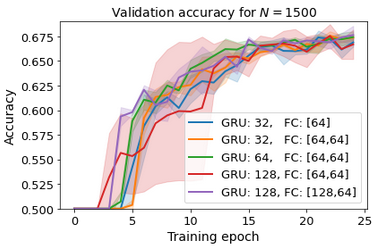
\includegraphics[width=0.4\linewidth]{Experiments/Figures/Hybrid/hybrid_architectures_identification.png}
    \caption{\red{[TODO: caption]}}
    \label{fig:hybrid-gru_architectures}
\end{figure}

\red{[TODO: provide table with test results]}
The classification accuracies of each model evaluated on the validation set during the process of training are plotted in Figure \ref{fig:hybrid-model_comparison}, from which several things can be noted. First of all, each model seems to perform worse in the case of longer ($N=1500$) light curve segments. This is probably due to the fact that the longer the segments, the more distracting background patterns may be present that mimic transit signals. The best performing models are GRU-based networks, which were not even trained for this specific task. The RNN that was trained specifically for this task, with a training procedure referred to as \textit{naive}, performed considerably worse. This is in line with our expectation that only providing a single learning signal to the RNN for a given input segment is bad practice. Lastly, we find that using more than one recurrent layer does not necessarily lead to better results. Therefore, in following experiments, we adopt a bidirectional GRU with a single recurrent layer (bi-GRU-1) that was trained on the data set with $N=1500$, and refer to this network simply as the "RNN".

\begin{figure}
    \centering
    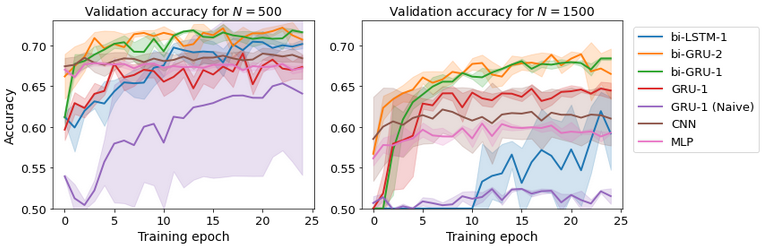
\includegraphics[width=0.8\linewidth]{Experiments/Figures/Hybrid/identification_models.png}
    \caption{\red{[TODO: caption]}}
    \label{fig:hybrid-model_comparison}
\end{figure}

\subsection{Locating signals in time for inputs of arbitrary size}

As opposed to the CNN and MLP, the RNN can handle arbitrary input sizes. This is illustrated in Figure \ref{fig:hybrid-pts}, where the RNN from Section \ref{sec:identification} is applied to a full-length light curve. In this case we show the RNN's output at each individual time step. Each peak in the resulting PTS indicates the presence of a potential transit signal at the corresponding time in the light curve. 

\begin{figure}
    \centering
    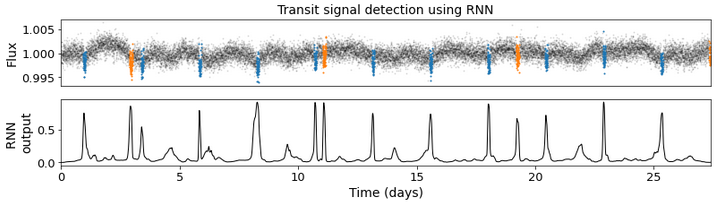
\includegraphics[width=0.8\linewidth]{Experiments/Figures/Hybrid/PTS_example.png}
    \caption{\red{[TODO: caption]}}
    \label{fig:hybrid-pts}
\end{figure}

However, data in the task of detection is less balanced than in the task of identification. This is because at the level of individual data points, we only have a few points that are labeled as signal, and many points that are labeled as non-signal. The accuracy of classification is therefore a misleading metric, as the network could already achieve high accuracies by classifying each data point as non-signal. Therefore we turn to different metrics for finetuning the network for detection. The true positive rate (TPR), or recall, is the fraction of the correctly classified positives (i.e. points labeled as signal). The true negative rate (TNR) is similar, but for correctly classified negatives instead of positives. Lastly, precision is the fraction of the samples classified as positive that were correct. 

If the classes were perfectly balanced, we expect a TPR similar to the TNR. In our LCSim data set with $N=1500$, we have 12.6 times more non-signal data points than points that are labeled as signal. Using an extra weight in the loss for transit points of $p_t=12.6$ will therefore balance our data set. Figure \ref{fig:hybrid-weighting} shows that this indeed the case. However, although tuning the TPR and TNR can be useful for our purposes, a lower TNR also means we falsely classify more samples as positive, thus decreasing the precision. To increase the recall, but avoid a large decrease in TNR we therefore adopt a smaller weight of $p_t=4$. The other weighting parameter that is varied, $w_i$, is used to tune how much each individual transit signal is weighted compared to others. For example, we can set $w_i = \delta_i / \sigma$, which will weigh each positive data point by its corresponding transit depth $\delta_i$ relative to the time-independent noise $\sigma$. In that case, a transit with twice the depth will get double the weight. This type of weighting might, however, cause the network to place too little focus on correctly detecting shallow transits. To reduce this effect, but still apply transit-specific weighting, we can adopt $w_i = \sqrt{\delta_i / \sigma}$. 


\begin{figure}
    \centering
    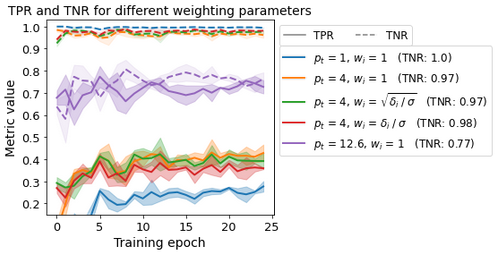
\includegraphics[width=0.5\linewidth]{Experiments/Figures/Hybrid/weighting_valid_lcsim.png}
    \caption{\red{[TODO: caption]}}
    \label{fig:hybrid-weighting}
\end{figure}

\begin{figure}
    \centering
    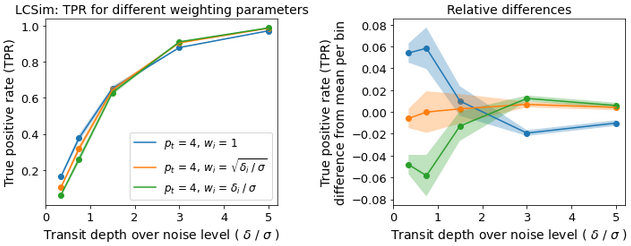
\includegraphics[width=0.65\linewidth]{Experiments/Figures/Hybrid/weighting_lcsim.png}
    \caption{\red{[TODO: caption]}}
    \label{fig:hybrid-lcsim_weighting}
\end{figure}

\begin{figure}
    \centering
    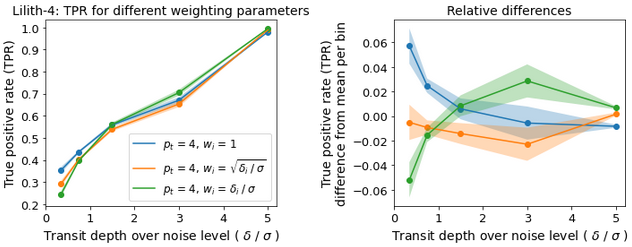
\includegraphics[width=0.65\linewidth]{Experiments/Figures/Hybrid/weighting_lilith.png}
    \caption{\red{[TODO: caption]}}
    \label{fig:hybrid-lilith_weighting}
\end{figure}

The effect of different weighting schemes on TPR and TNR are visualized in Figure \ref{fig:hybrid-weighting}. Figures \ref{fig:hybrid-lcsim_weighting} and \ref{fig:hybrid-lilith_weighting} show the TPR against different relative transit depths, which was evaluated of test splits both data sets.
\todo{describe how Lilith-4 light curve segments were obtained.} In the following experiments, we adopt $p_t=4$ and $w_i = \sqrt{\delta_i / \sigma}$, unless stated otherwise.

